%

\section{Impossibility Theorems}\label{sec:impossibility}

Our main result is that \textbf{for mildly rich \modelname{} classes, it is impossible to conclude that the \username{} does better than random guessing at inferring \countmodbehaviourname{} using common \fielddefnames{} without strong additional assumptions on the learning algorithm or data distribution.}
We also apply this result to two common \downtasknames{}, showing that under these conditions, it is impossible to conclude that the \username{} does better than random guessing for algorithmic recourse and spurious \covname{} identification using these \fielddefnames{}.
Finally, we show that even for very simple \modelnames{} (so our richness condition does not hold), these \fielddefnames{} provably still incorrectly infer \countmodbehaviourname{} with significant probability.
%
%
%

To characterize the common \fielddefnames{} we consider, we begin by defining two commonly used properties of such methods: \emph{\completenames{}} and \emph{\additivenames{}}.
Informally, \completenames{} requires that the individual \covname{} \attnames{} sum to the difference of the \modelname{} output from the \basename{}, while \additivenames{} requires that if the \modelname{} has no \covname{} interactions then the \attnames{} of a given \covname{} should be equivalent to considering that \covname{} on its own. 

\begin{definition}[\completeName{}]\label{defn:complete}
A \fielddefname{}
$\expdef$ is \emph{\completename{}} if and only if
for all
\modelnames{} $\model\in\modelspace$,
\basenames{} $\covdist\in\probspace(\covspace)$,
and
\obsnames{} $\covval\in\covspace$,
%
%
%
%
\*[
    \sum_{j\in[\covdim]}\expdef(\model,\covdist,\covval)\feat{j}
    = \model(\covval) - \EE_{\covobs\sim\covdist} \model(\covobs).
\]
\end{definition}

\begin{definition}[\additiveName{}]\label{defn:additive}
A \fielddefname{}
$\expdef$ is \emph{\additivename{}} if and only if
for all collections of functions $\model^{(1)},\dots,\model^{(\covdim)}:\Reals\to\dataspace$,
if $\model(\covval) = \sum_{j\in[\covdim]} \model^{(j)}(\covval\feat{j}) \in \modelspace$ then for all \basenames{} $\covdist\in\probspace(\covspace)$, \obsnames{} $\covval\in\covspace$, and \covnames{} $j\in[\covdim]$
%
\*[
    \expdef(\model,\covdist,\covval)\feat{j}
    = \expdef(\model\feat{j},\covdist\feat{j},\covval\feat{j}).
\]
\end{definition}

%


Two of the most common \fielddefnames{}, \shap{} \citep{lundberg17shapley} and \intgrad{} \citep{sundararajan17integrated}, are \completename{} and \additivename{} (for precise definitions and statements, see \cref{sec:complete-additive-proofs}).

\subsection{Assumptions on the \modelName{} }

Our theoretical results rely on two mild assumptions about the \covnames{} and the \modelname{} class.
These assumptions are typically satisfied in the cases we are interested in: neural networks applied beyond toy problems. %
This implies that to
%
do better than random guessing with common \fielddefnames{}, the \username{} must necessarily introduce more structure than this standard setting.

\paragraph{\cref{assn:inscale-covdist} \intuitive{}}
This assumption has two parts.
First, we require that $\covspace$ is not degenerate near $\covval$; i.e., there exists an interval around $\covval$ on which we can study \countmodbehaviourname{}.
If this were not true, it would not make sense to ask about the \modbehaviourname{} \scarequo{near $\covval$} (encoded by $\inscale$ as described in \cref{sec:counterfactual}).
%
In particular, we restrict ourselves to continuous input spaces. For sufficiently rich discrete input spaces (i.e., taking more than a few distinct values), our results could be proved in the same way with more notational overhead.
%

%
Second, we require that the \basename{} has support outside of this interval.
%
%
This assumption is mild in practice.
For example, when the \basename{} is the training distribution, there only needs to be a single training example that does not fall in the interval above.
When the \basename{} concentrates on a single \obsname{}, this \obsname{} must fall outside of the interval; in this case, the \basename{} \obsname{} usually corresponds to setting all features to zero, or all pixels to black, and hence is sufficiently far from any $\covval$ of interest. We formalize this as follows.

\begin{assumption}\label{assn:inscale-covdist}
For any \obsname{} $\covval\in\covspace$, \covname{} $j\in[\covdim]$, \radiusname{} $\inscale>0$, and \basename{} $\covdist\in\probspace(\covspace)$, we say that the present assumption holds if there exist $\covleft\feat{j},\covright\feat{j}\in\Reals$ such that
\*[\label{eqn:inscale-covdist}
    [\covval\feat{j}-\inscale,\covval\feat{j}+\inscale] \subseteq (\covleft\feat{j},\covright\feat{j}) \subseteq \{\covvaldum\feat{j}\setdelim\covvaldum\in\covspace\}
\]
and
\*[
    \covdist\feat{j}\Big((\covleft\feat{j}, \covright\feat{j}) \setminus [\covval\feat{j}-\inscale\feat{j}, \covval\feat{j}+\inscale\feat{j}]\Big) > 0.
\]
\end{assumption}


%
\paragraph{\cref{assn:piecewise} \intuitive{}}
General impossibility results are unobtainable; for example, most \fielddefnames{} correctly identify the \modelname{} for linear models. In other words, to derive an implication similar to ours (that the \covname{} \attname{} does not provide information about \countmodbehaviourname{}) one must impose some constraint on the \modelname{} class.
The purpose of this assumption is to define how rich a model would have to be for our result to hold. Note that this assumption
%
includes standard machine learning architectures such as neural networks with reasonable complexity.
%
%

In particular, we require that the \modelname{} class $\modelspace$ can represent sufficiently many piecewise linear extensions of the \localname{} \countmodbehaviourname{} (encoded by $\modeldum$ as described in \cref{sec:counterfactual}) that the \username{} wishes to infer.
This is naturally satisfied by ReLU networks: every ReLU network is a piecewise linear function, and any ReLU network of logarithmic (in dimension) depth or polynomial (in number of pieces) size can exactly replicate any piecewise linear function \citep[for precise bounds, see][]{arora18relu,tanielian21groupsort,chen22piecewise}.
This does not preclude the \modelname{} class from being arbitrarily richer than piecewise linear functions.


To precisely describe \cref{assn:piecewise}, we need some standard notation.
For any neighbourhood $\covnbhd\subseteq\covspace$ and \modelname{} $\model:\covspace\to\dataspace$, let $\model\restrict{\covnbhd}$ be the \modelname{} restricted to have the domain $\covnbhd$; that is, $\model\restrict{\covnbhd} = (\covnbhd\ni\covval\mapsto\model(\covval))$.
Similarly, let $\modelspace\restrict{\covnbhd} = \{\model\restrict{\covnbhd}\setdelim\model\in\modelspace\}$ denote the collection of all such restrictions.
We say that $\model$ is a \emph{$\numpiece$-piecewise linear function on $\covnbhd\subseteq\covspace$} if there exist closed, convex polytopes $\polytope\feat{1},\dots,\polytope\feat{\numpiece}$ that partition $\covnbhd$ such that $\model\restrict{\polytope\feat{j}}$ is linear for each $j\in[\numpiece]$ and $\model$ is continuous.
%
This is a standard definition, for example, see Definition~1 of \citet{chen22piecewise}.
Let $\pwiselin{\numpiece}\restrict{\covnbhd}$ denote the set of all $\numpiece$-piecewise linear elements of $\covnbhd\to\dataspace$.
%
We place the following assumption on the minimum richness of the \modelname{} class.
%

\begin{assumption}\label{assn:piecewise}
For any \obsname{} $\covval\in\covspace$, \covname{} $j\in[\covdim]$, \radiusname{} $\inscale>0$,
and \modbehaviourname{} $\modeldum:[\covval\feat{j}-\inscale, \covval\feat{j}+\inscale]\to\dataspace$,
we say that the present assumption holds if for the neighbourhood $\covnbhd = [\covval\feat{j}-\inscale, \covval\feat{j}+\inscale] \times \covspace\feat{[\covdim]\setminus\{j\}}$,
\*[
    \Big\{\model:
    \forall \covvaldum\in\covnbhd \ \model(\covvaldum) = \modeldum(\covvaldum\feat{j}), \ \model\restrict{\comp{\covnbhd}} \in \pwiselin{2}\restrict{\comp{\covnbhd}}\Big\} \subseteq \modelspace.
\]
%
\end{assumption}

%
%
%
%
If the \modbehaviourname{} $\modeldum$ is piecewise linear, then \cref{assn:piecewise} is satisfied by any $\modelspace$ expressive enough to realize piecewise linear functions.
If the \pracname{} is interested in \modbehaviourname{} that is more complex than piecewise linear, then it is reasonable to assume that $\modelspace$ is sufficiently expressive to represent this more complex \modbehaviourname{} locally, and thus \cref{assn:piecewise} is again satisfied if the \modelname{} class includes piecewise linear functions away from the region of interest.


\subsection{Main Result}

\begin{theorem}\label{fact:oracle-hypothesis}
Fix any \obsname{} $\covval\in\covspace$, \covname{} $j\in[\covdim]$,
\radiusname{} $\inscale>0$,
\basename{} $\covdist \in \probspace(\covspace)$,
and
\modbehaviourname{} $\modeldum\nullind,\modeldum\altind:[\covval\feat{j}-\inscale, \covval\feat{j}+\inscale]\to\Reals$.
Suppose that \cref{assn:inscale-covdist,assn:piecewise} are satisfied.
Let
\*[
    \modelspace\nullind
    &= \Big\{\model\in\modelspace\setdelim \forall\covvaldum\feat{j}\in[\covval\feat{j}-\inscale,\covval\feat{j}+\inscale], \ \model(\covval\feat{[\covdim]\setminus\{j\}},\covvaldum\feat{j}) = \modeldum\nullind(\covvaldum\feat{j}) \Big\} \\
    \modelspace\altind
    &= \Big\{\model\in\modelspace\setdelim \forall\covvaldum\feat{j}\in[\covval\feat{j}-\inscale,\covval\feat{j}+\inscale], \ \model(\covval\feat{[\covdim]\setminus\{j\}},\covvaldum\feat{j}) = \modeldum\altind(\covvaldum\feat{j}) \Big\}.
\]
For any \completename{} and \additivename{} \fielddefname{} $\expdef$ and $\oraclehyptest:\Reals^{\covdim\times\datadim}\to[0,1]$,
\*[
    \specsym_{\expdef,\covdist,\covval}(\oraclehyptest) \leq 1 -
    \senssym_{\expdef,\covdist,\covval}(\oraclehyptest).
\]
\end{theorem}

%
To interpret this result, consider that for any $\covprob\in[0,1]$, the trivial \hyptestname{} $\oraclehyptest \equiv \covprob$ that ignores the \modelname{}
%
will achieve
\*[
    \specsym_{\expdef,\covdist,\covval}(\oraclehyptest)
    = 1 - \senssym_{\expdef,\covdist,\covval}(\oraclehyptest).
\]
We refer to this family of trivial tests as \emph{random guessing}.
For example, one can always achieve $\specsym_{\expdef,\covdist,\covval}(\oraclehyptest) = 0$ at the expense of $\senssym_{\expdef,\covdist,\covval}(\oraclehyptest) = 1$ (by always rejecting the \nullname{}) or $\specsym_{\expdef,\covdist,\covval}(\oraclehyptest) = \senssym_{\expdef,\covdist,\covval}(\oraclehyptest) = 0.5$ (by ignoring the data and using a coin flip).
\cref{fact:oracle-hypothesis} shows that the best tradeoff between \sensname{} and \specname{} that can be achieved by \completename{} and \additivename{} \fielddefnames{} is no better than the tradeoff achieved by random guessing.
In other words, this result says that without imposing additional assumptions on the underlying data or learning algorithm to significantly reduce the \modelname{} complexity, the \username{} cannot conclude that they have learned any information about the \modelname{}.
In particular, they may do no better than random guessing at \downtasknames{} such as recourse and spurious \covname{} identification. %
In \cref{sec:experiments}, we demonstrate that this holds empirically for real data and real models.

For simplicity, we state our results for \countmodbehaviourname{} with respect to how the \modelname{} depends on a single \covname{} at a time, and defer the extension to arbitrary groups of \covnames{} as well as all proofs to \cref{sec:impossibility-proofs}.
The generality of \cref{fact:oracle-hypothesis} means that it applies to inferring any form of \countmodbehaviourname{}.
Returning to the clinical trial setting
of \citet{liu21oncology} in the introduction, the \username{} may wish to infer if the \modelname{} output changes as a function of a certain \covname{} (e.g., is the hazard ratio sensitive to the exclusion criteria).
To answer this, they must be able to distinguish between $\modeldum\nullind \equiv 0$ and some $\modeldum\altind$ that changes with \covname{} $j$.
However, \cref{fact:oracle-hypothesis} implies that for every such $\modeldum\altind$, the \username{} cannot conclude that they do better than random guessing at this inference task, and therefore, at identifying whether the \modelname{} depends on the \covname{}.
Thus, if this method is used for purposes such as determining membership in a clinical trial, the conclusions are not guaranteed to be any more reliable than random guessing. This has significant implications for using such methods in safety-critical or high stakes applications.

%

\subsection{Proof Sketch of \cref{fact:oracle-hypothesis}}\label{sec:proof-sketch}

The primary technical result (proved in \cref{sec:impossibility-proofs}) that facilitates our results is:

%
\begin{theorem}\label{fact:interior-freedom}
Fix any \obsname{} $\covval\in\covspace$, \covname{} $j\in[\covdim]$, 
%
\radiusname{} $\inscale>0$,
\basename{} $\covdist \in \probspace(\covspace)$, 
and
\modbehaviourname{} $\modeldum:[\covval\feat{j}-\inscale, \covval\feat{j}+\inscale]\to\dataspace$.
Suppose that \cref{assn:inscale-covdist,assn:piecewise} are satisfied. 
%
For every \attname{} $\expval \in \Reals^{\datadim}$, there exists 
a \modelname{} $\model\in\modelspace$ such that for every \completename{} and \additivename{} \fielddefname{}, $\expdef(\model,\covdist,\covval)\feat{j} = \expval$, and if $\abs[0]{\covval\feat{j}-\covvaldum\feat{j}} \leq \inscale\feat{j}$ then $\model(\covvaldum) = \modeldum(\covvaldum\feat{j})$.
\end{theorem}

Equipped with \cref{fact:interior-freedom}, we use it to prove \cref{fact:oracle-hypothesis} by constructing a counterexample. For any \nullname{} $\modelspace\nullind$ and \altname{} $\modelspace\altind$, we choose $\modeldum\nullind$ and $\modeldum\altind$ satisfying the \countmodbehaviourname{} prescribed by the \nullname{} and \altname{} respectively. For example, in the recourse setting, $\modeldum\nullind$ may be increasing in the \covname{} while $\modeldum\altind$ is decreasing.
%
Then, by \cref{fact:interior-freedom}, we can construct $\model\nullind$ and $\model\altind$ that locally agree with $\modeldum\nullind$ and $\modeldum\altind$ respectively, yet receive the same \covname{} \attname{}. Consequently, any \oraclehyptestname{} that relies on only the \covname{} \attname{} to draw conclusions cannot distinguish between $\model\nullind$ and $\model\altind$, and hence has been provided no additional information to do better than random guessing.
While a single counterexample is sufficient to prove \cref{fact:oracle-hypothesis}, the proof of \cref{fact:interior-freedom} reveals that we can actually find uncountably many \modelnames{} that work as counterexamples, which has important implications for practical settings.
We demonstrate this in our on-average results (\cref{sec:average-behaviour}) and experiments (\cref{sec:experiments}).

We visualize the intuition behind this result in \cref{fig:attribution}, where we show (a) \modelnames{} can behave very differently and all receive the same attribution and (b) \modelnames{} can be identical in a local neighbourhood of interest yet receive very different attribution. 
%
Critically, our counterexamples are very simple (piecewise linear in the proof, piecewise quadratic for smooth visualization in \cref{fig:attribution}), and hence easily realized by neural networks.
Finally, since \fielddefnames{} provide only a summary of the \modelname{}, it is clear that one can always find \emph{some} example of two different \modelnames{} that receive the same \attname{}.
The primary insight that enables our results is that we can always find \modelnames{} that \emph{differ in exactly the way that we wish to test} yet receive the same \attname{}. The next natural question is: how does this result extend to \downtasknames{} that practitioners care about?


%
%
%
%
%
%
%
%
%
%
%
%
%

\begin{figure}
\centering
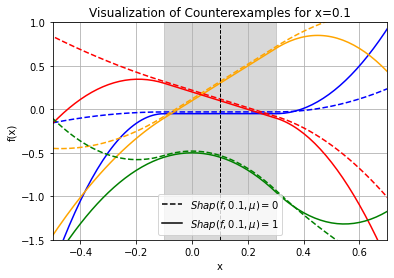
\includegraphics[scale=0.6]{figure-files/joint-att.png}
    \caption{Each line represents a different one-dimensional \modelname{}. For $\covval=0.1$ and $\covdist=\uniformdist(-1,1)$, dashed lines receive \shap{}$(\model,\covval,\covdist)=0$ while solid lines receive \shap{}$(\model,\covval,\covdist)=1$. The behaviour of models with the same colour is identical within the shaded region, which denotes the neighbourhood $(\covval-\inscale,\covval+\inscale)$ for $\inscale=0.2$. \modelNames{} can behave very differently and all receive the same \attname{} (e.g., all dashed lines) and \modelnames{} can be identical in a neighbourhood yet receive very different \attname{} within that neighbourhood (e.g., lines with the same colour). }
    \label{fig:attribution}
\end{figure}
%
%
%
%

%
%
%
%
%

\subsection{Results for \downtaskNAMEs{} of Interest}

We discuss three \downtasknames{}, starting with the simplest one (\localname{} \modbehaviourname{}) which forms the basis of the two more common \downtasknames{}: recourse and spurious correlation.
There are multiple notions of these \tasknames{} in the literature, and they are often used without a precise formalization.
To facilitate analysis, we provide \emph{one possible} formalization of the easiest version of these \tasknames{}.
We defer general definitions and full proofs to \cref{sec:application-proofs}.
%

\subsubsection{Simple \localName{} \modbehaviourNAME{}}\label{sec:local-behaviour}

%
A consequence of \cref{fact:oracle-hypothesis} is that if the notion of \countmodbehaviourname{} is sufficiently local,
%
\shap{} and \intgradshort{} may not provide valid inference for $\model$. Specifically, we consider the task of identifying whether a \modelname{} output is locally sensitive to perturbations of a \covname{}, which is a necessary component of identifying spurious features: if one can reliably identify spurious features, one must be able to identify \covnames{} for the which the \modelname{} output is insensitive to small perturbations. We first show that \vanillagrad{} is \emph{always} successful at this \taskname{} for a sufficiently small notion of perturbations.
While the limitations of \vanillagrad{} are well-known for many \tasknames{} \citep{adebayo18sanity} and there are additional challenges for \vanillagrad{} computed using backpropagation \citep{nie18backprop}, the following result demonstrates that there exists a \taskname{} for which \vanillagrad{} is reliable yet \shap{} and \intgradshort{} may not be.
%

\begin{proposition}\label{fact:local-stability-grad}
Fix $\covval\in\covspace$ and suppose $\modelspace \subseteq \{\model: \Reals^\covdim \to \Reals, \grad\model(\covval) \ \mathrm{ exists }\}$.
For every $\outscale>0$, $\covval\in\covspace$, and $j\in[\covdim]$, there exists $\inscale>0$ such that if
\*[
    %
    %
    \modelspace\nullind
    &= \Big\{\model\in\modelspace: \sup_{\alpha\leq\inscale} \abs{\model(\covval+\alpha e_j) - \model(\covval)} \leq \inscale \outscale / 2 \Big\} \\
    \modelspace\altind
    &= \Big\{\model\in\modelspace: \sup_{\alpha\leq\inscale} \abs{\model(\covval+\alpha e_j) - \model(\covval)} > \inscale \outscale \Big\},
\]
then there exists $\oraclehyptest$ using $\expdef=$ \vanillagrad{} such that for every $\covdist\in\probspace(\covspace)$
\*[
    \specsym_{\expdef,\covdist,\covval}(\oraclehyptest)
    = \senssym_{\expdef,\covdist,\covval}(\oraclehyptest)
    = 1.
\]
\end{proposition}

Using \cref{fact:oracle-hypothesis}, we next show that \completename{} and \additivename{} \fieldmethodnames{} provably are less reliable than \vanillagrad{} for this task.

\begin{proposition}\label{fact:local-instability}
Fix $\covval\in\covspace$ and suppose $\{\model: \Reals^\covdim \to \Reals, \model \ \text{\upshape is piecewise linear and }  \grad\model(\covval) \ \mathrm{ exists }\} \subseteq \modelspace \subseteq \{\model: \Reals^\covdim \to \Reals, \grad\model(\covval) \ \mathrm{ exists }\}$.
For every sufficiently small $\outscale,\inscale>0$, $\covval\in\covspace$, and $j\in[\covdim]$, if
\*[
    \modelspace\nullind
    &= \Big\{\model\in\modelspace: \sup_{\alpha\leq\inscale} \abs{\model(\covval+\alpha e_j) - \model(\covval)} \leq \inscale \outscale/2 \Big\} \\
    \modelspace\altind
    &= \Big\{\model\in\modelspace: \sup_{\alpha\leq\inscale} \abs{\model(\covval+\alpha e_j) - \model(\covval)} > \inscale \outscale \Big\},
\]
then for every \oraclehyptestname{} $\oraclehyptest$, \completename{} and \additivename{} \fielddefname{} $\expdef$, and $\covdist\in\probspace(\covspace)$ satisfying \cref{assn:inscale-covdist},
\*[
    \specsym_{\expdef,\covdist,\covval}(\oraclehyptest)
    \leq 1 - \senssym_{\expdef,\covdist,\covval}(\oraclehyptest).
\]
\end{proposition}

\subsubsection{Recourse and Spurious \covNames{}}\label{sec:downtasks}

While \cref{sec:local-behaviour} proves that \completename{} and \additivename{} \fielddefnames{} can be unreliable for inferring sufficiently local \countmodbehaviourname{}, common \downtasknames{} in the literature are only \scarequo{moderately} local.
%
We now show that inference for these \tasknames{} can also be as uninformative as random guessing.
To do so,
we formalize increasing and decreasing a \covname{} by considering a distribution over perturbations and measuring the \modelname{} change on average with respect to this distribution (which may differ from the \basename{} used to compute the \covname{} \attname{}).
%

\begin{definition}[Recourse]\label{defn:recourse}
Fix any $\covval\in\covspace$, $j\in[\covdim]$, $k\in[\datadim]$,
$\inscale >0$, and
$\covdistdum \in \probspace(\covspace)$.
Let
\*[
    \modelspace\nullind
    &= \Big\{
    \model\in\modelspace\setdelim \EE_{\covobs\sim\covdistdum}\Big[\model(\covval\feat{[\covdim]\setminus\{j\}}, \covobs\feat{j})\feat{k} \condsym \covobs\feat{j} \in [\covval\feat{j}, \covval\feat{j}+\inscale]\Big] \\
    &\hspace{16mm}> \EE_{\covobs\sim\covdistdum}\Big[\model(\covval\feat{[\covdim]\setminus\{j\}}, \covobs\feat{j})\feat{k} \condsym \covobs\feat{j} \in[\covval\feat{j}-\inscale,\covval\feat{j}]\Big]\Big\} \\
    \modelspace\altind
    &= \modelspace \setminus \modelspace\nullind.
\]
\end{definition}

\paragraph{Recourse \intuitive{}}
Here, $\covdistdum$ is a distribution from which perturbed \obsnames{} can be sampled from.
This distribution need not be the same as the \basename{} used by the \fielddefname{}---a common choice would be the uniform distribution or a pointmass for a single perturbation of interest.
Then, $\modelspace\nullind$ corresponds to those \modelnames{} where increasing \covname{} $j$ will increase the \modelname{} output on average.
Again as a concrete example, if the \modelname{} output is the probability of loan acceptance and \covname{} $j$ is income, the \pracname{} asks whether to increase or decrease credit score in order to improve the probability of acceptance.

Next, we formalize distinguishing whether a \modelname{} is sensitive or insensitive to perturbations.
%

\begin{definition}[Spurious \covNames{}]\label{defn:spurious}
Fix any $\covval\in\covspace$, $j\in[\covdim]$, $k\in[\datadim]$,
$\inscale >0$, and $\outscale>0$.
Let
\*[
    \modelspace\nullind &= \Big\{\model\in\modelspace \setdelim \sup_{\covvaldum\feat{j}\in(\covval\feat{j},\covval\feat{j}+\inscale]} \abs[0]{\model(\covval\feat{[\covdim]\setminus\{j\}},\covvaldum\feat{j})\feat{k}} \, = 0\Big\} \\
    \modelspace\altind &= \Big\{\model\in\modelspace \setdelim \sup_{\covvaldum\feat{j}\in(\covval\feat{j},\covval\feat{j}+\inscale]} \abs[0]{\model(\covval\feat{[\covdim]\setminus\{j\}},\covvaldum\feat{j})\feat{k}} \, \geq \outscale\Big\}.
\]
%
\end{definition}

\paragraph{Spurious \covNames{} \intuitive{}}
$\modelspace\nullind$ corresponds to those \modelnames{} where the \modelname{} output does not change from perturbing \covname{} $j$.
Meanwhile, $\modelspace\altind$ corresponds to the \modelnames{} that have a \scarequo{significant} change from perturbing \covname{} $j$, where
significance is encoded by the size of $\outscale$.
Concretely, if \covnames{} correspond to the pixels of a watermark on an X-ray, the \pracname{} asks whether the \modelname{} output is sensitive to the values of these pixels.

%

We now apply \cref{fact:oracle-hypothesis} to these definitions and obtain the following implications.
%
%

\begin{corollary}\label{fact:oracle-hypothesis-examples}
Fix any $\covval\in\covspace$, $j \in [\covdim]$,
$\inscale>0$,
and $\covdist\in\probspace(\covspace)$ such that \cref{assn:inscale-covdist} is satisfied.
Fix
$k\in[\datadim]$ and
$\covdistdum \in \probspace(\covspace)$,
and
let $\modelspace\nullind$ and $\modelspace\altind$ be as defined in either \cref{defn:recourse} or \cref{defn:spurious}.
%
Suppose that there exists $\model\nullind\in\modelspace\nullind$ and $\model\altind\in\modelspace\altind$ such that $\modeldum\nullind = \model\nullind\restrict{\covnbhd}$ and $\modeldum\altind = \model\altind\restrict{\covnbhd}$ each satisfy \cref{assn:piecewise}.
Then
for any \completename{} and \additivename{} \fielddefname{} $\expdef$ and \oraclehyptestname{} $\oraclehyptest$,
\*[
    \specsym_{\expdef,\covdist,\covval}(\oraclehyptest) \leq 1 -
    \senssym_{\expdef,\covdist,\covval}(\oraclehyptest).
\]
\end{corollary}

As previously mentioned, \cref{fact:oracle-hypothesis-examples} implies that the \pracname{} cannot distinguish whether increasing or decreasing the \covname{} is the correct direction to increase the \modelname{} prediction.
For recourse, the main assumption that \cref{assn:piecewise} holds is satisfied in this case when $\modelspace$ contains piecewise linear functions, since the functions $\modeldum(\covval\feat{j}) = \covval\feat{j}$ for $\model\nullind$ and
$\modeldum(\covval\feat{j}) = -\covval\feat{j}$ for $\model\altind$ suffice.
Similarly, \cref{fact:oracle-hypothesis-examples} implies that the \pracname{} cannot distinguish whether the \modelname{} prediction is sensitive to changes in the \covname{}.
For spurious features, the main assumption that \cref{assn:piecewise} holds is again satisfied when $\modelspace$ contains piecewise linear functions, since the functions $\modeldum(\covval\feat{j}) = 0$ for $\model\nullind$ and
$\modeldum(\covval\feat{j}) = \outscale$ for $\model\altind$ suffice.

%
%
%
%
%
%
%
%
%
%
%
%
%
%
%
%
%
%


\subsection{Average \localName{} Performance for Simple \modelNames{}}\label{sec:average-behaviour}

As motivated in \cref{sec:notation}, the usual definitions of \specname{} and \sensname{} demand accurate \hyptestnames{} for every \modelname{} of interest. We now show that for standard distributions placed over simple \modelname{} classes, our results apply even for the \emph{easier} task of obtaining accurate \hyptestnames{} on average over the models.

Consider the simple class of univariate \modelnames{} $\modelspace = \{\covval\mapsto a \covval^n - \covval \setdelim a\in\Reals\}$ for some fixed $n \geq 2$. Although this \modelname{} class is so simple that \cref{assn:piecewise} does not apply (and hence we cannot directly apply \cref{fact:oracle-hypothesis}), we can prove a similar result that applies on average.

\begin{proposition}\label{fact:random-quadratic}
Let $\pi$ denote the distribution over $\modelspace$ induced by $a \sim \normaldist(0,1)$, let $\covdist$ be such that $\EE_\covdist \covobs^n \in (1/2,1)$, and set $\covval=1$. Then, for any \completename{} and \additivename{} $\expdef$,
\*[
    \PP_{\model\sim\pi}\Big[\sgn(\expdef(\model,\covdist,\covval)) \neq \sgn(\model'(\covval)) \Big] \in (0.25, 0.5).
\]
\end{proposition}

As a consequence, any \oraclehyptestname{} that relies on the sign of a \completename{} and \additivename{} \fielddefname{} to infer \localname{} \countmodbehaviourname{} will draw the wrong conclusion at least 1/4 of the time, even for this exceedingly simple model class.
In the next section, we show empirically that our results apply on average in the more complex settings for which \cref{fact:oracle-hypothesis} applies.

%
